\documentclass[11pt]{article}
\usepackage{preamble}
\titleformat*{\section}{\Large\bfseries}

\title{CISC 3220 Homework}
\author{Rachel Friedman}
\date{March 22, 2020}

\begin{document}
\maketitle

\section*{Problem 4.5-1 a}\nointerlineskip
\noindent \rule{\linewidth}{0.01pt}\\
\begin{flalign*}
T(n) = 2 T(n/4) + 1\\
&a = 2\\
&b = 4\\
&f(n) =1\\
&n^{log_b a} = n^{log_4 2} = n^{0.5} \\
\text{Case 1: }  &f(n)=\mathcal{O}(n^{log_b a-\epsilon})\\
& 0 \leq 1 \leq c \cdot n^{.5-\epsilon}\\
&\text{Let } \epsilon = .1\\
\text{For all asymptotically positive functions, there is a c such that: } &0 \leq 1 \leq c \cdot n^{.4}\\
&\text{So } T(n) = \Theta(n^{0.5})\\
\text{Thus, } & c_1 \cdot n^{0.5} \leq 2 T(n/4) + 1 \leq c_2 \cdot n^{0.5}\\
&\text{Let } c_1=1\\
&\text{Let } c_2=???\\
\color{red}\text{I can't seem to find a value for $c_2$ here that is not dependent on $n$.} \\
\color{red}\text{What am I doing wrong?? Using 10 for now.}\\
\end{flalign*}
\begin{center}
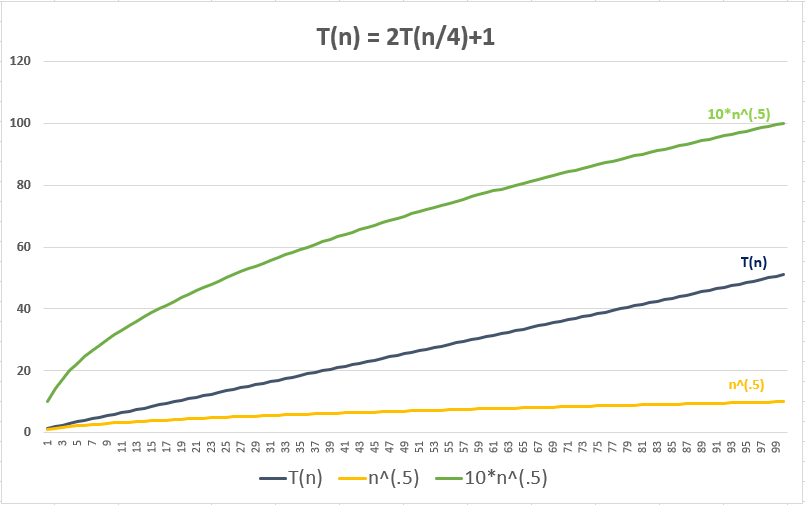
\includegraphics[scale=.6]{451a_.png}\\
\end{center}

\section*{Problem 4.5-1 b}\nointerlineskip
\noindent \rule{\linewidth}{0.01pt}\\
\begin{flalign*}
T(n) = 2 T(n/4) + \sqrt{n}\\
&a = 2\\
&b = 4\\
&f(n) = \sqrt{n}\\
&n^{log_b a} = n^{log_4 2} = n^{0.5} \\
\text{Case 2: }  &f(n)=\Theta(n^{log_b a})\\
&\text{So } T(n) = \Theta(n^{0.5} \text{ lg } n)\\
\text{Thus, }  c_1 \cdot n^{0.5} \text{ lg } n &\leq 2 T(n/4) + \sqrt{n} \leq c_2 \cdot n^{0.5} \text{ lg } n\\
&\text{Let } c_1=1\\
&\text{Let } c_2=???\\
\color{red}\text{I can't seem to find a value for $c_2$ here that is not dependent on $n$.} \\
\color{red}\text{What am I doing wrong?? Using 5 for now.}\\
\end{flalign*}
\begin{center}
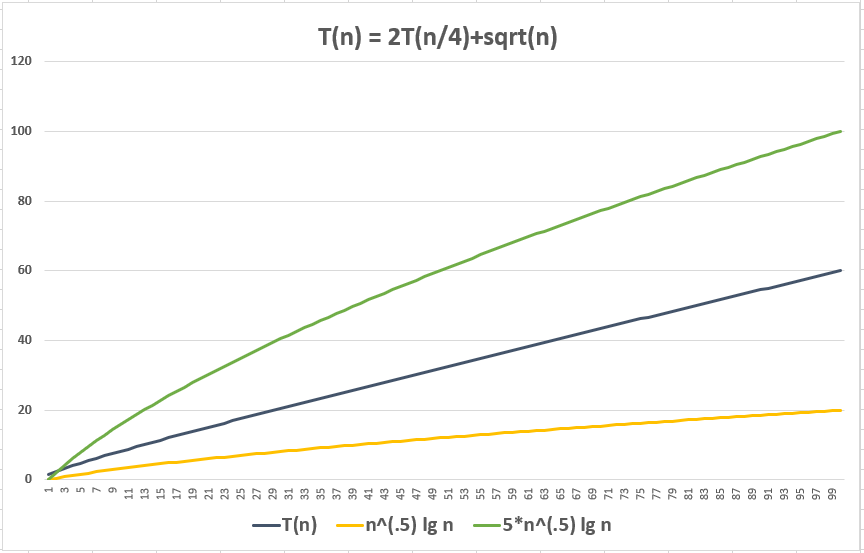
\includegraphics[scale=.6]{451b_.png}\\
\end{center}

\section*{Problem 4.5-1 c}\nointerlineskip
\noindent \rule{\linewidth}{0.01pt}\\
\begin{flalign*}
T(n) = 2 T(n/4) +n\\
&a = 2\\
&b = 4\\
&f(n) = n\\
&n^{log_b a} = n^{log_4 2} = n^{0.5} \\
\text{Case 3: }  &f(n)=\Omega(n^{log_b a+\epsilon})\\
&0 \leq n \geq n^{0.5 + \epsilon}\\
&\text{Let } \epsilon=.1\\
&n \geq n^{.6}\\
\text{Check regularity condition: }\\
\text{Find a c less than 1 for all sufficiently large n, such that: }\\
& 2  \frac{n}{4} \leq c_2 \cdot n\\
&\text{Let } c = \frac{1}{2}\\
\text{So } &T(n) = \Theta(n)\\
&c_1 n \leq 2 T(n/4) +n \leq c_2 n\\
&\text{Let } c_1=1\\
&\text{Let } c_2=2\\
\end{flalign*}
\begin{center}
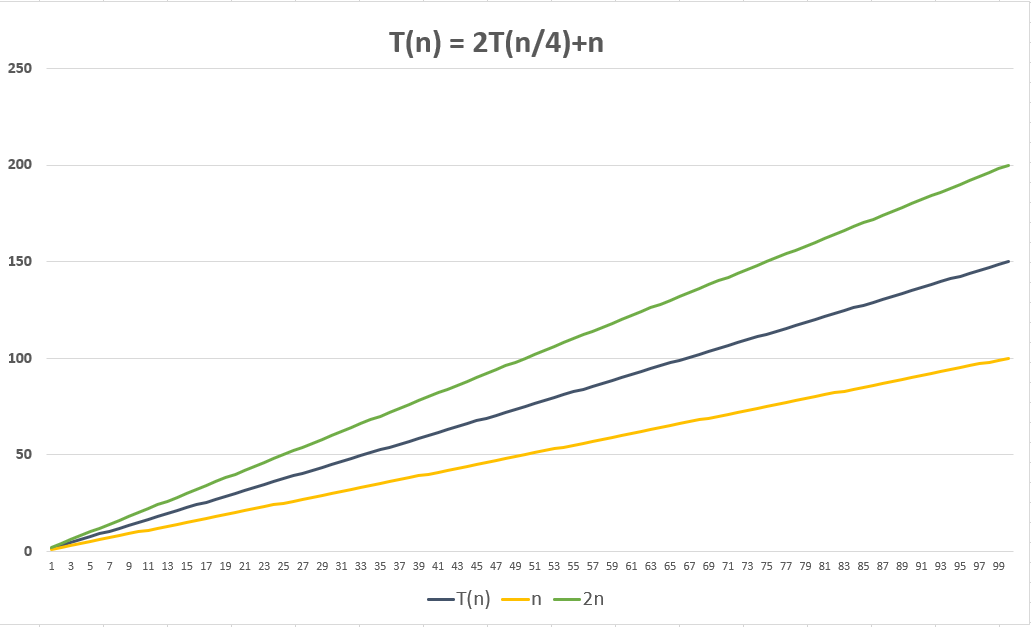
\includegraphics[scale=.6]{451c_.png}\\
\end{center}

\section*{Problem 4.5-1 d}\nointerlineskip
\noindent \rule{\linewidth}{0.01pt}\\
\begin{flalign*}
T(n) = 2 T(n/4) +n^2\\
&a = 2\\
&b = 4\\
&f(n) = n^2\\
&n^{log_b a} = n^{log_4 2} = n^{0.5} \\
\text{Case 3: }  &f(n)=\Omega(n^{log_b a+\epsilon})\\
&0 \leq n^2 \geq n^{0.5 + \epsilon}\\
&\text{Let } \epsilon=.1\\
&n^2 \geq n^{.6}\\
\text{Check regularity condition: }\\
\text{Find a c less than 1 for all sufficiently large n, such that: }\\
& 2  \frac{n}{4} \leq c \cdot n^2\\
&\text{Let } c = \frac{1}{2}\\
\text{So } &T(n) = \Theta(n^2)\\
&c_1 n^2 \leq 2 T(n/4) +n^2 \leq c_2 n^2\\
&\text{Let } c_1=0.5\\
&\text{Let } c_2=2\\
\end{flalign*}
\begin{center}
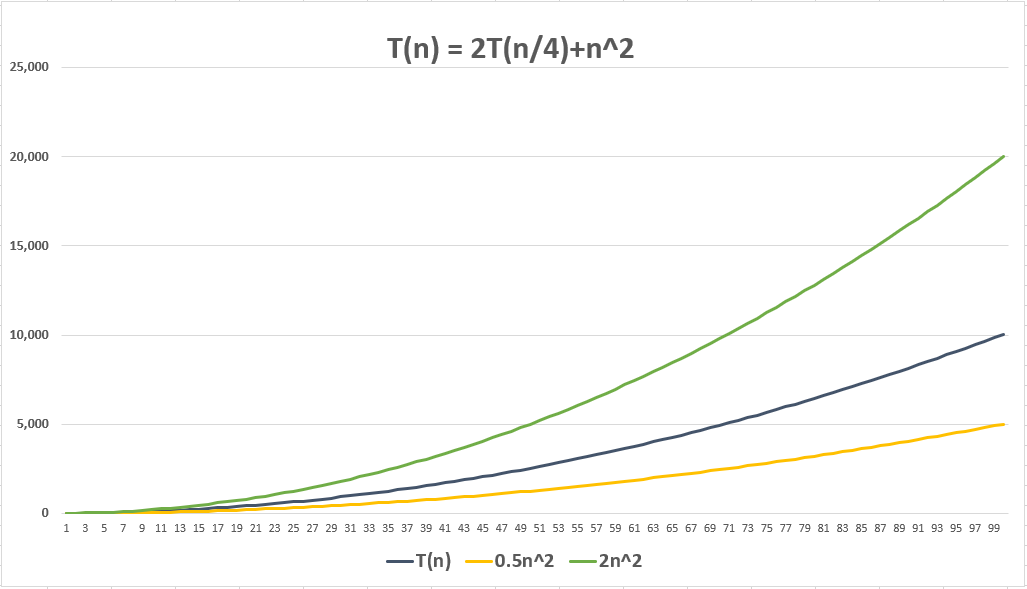
\includegraphics[scale=.6]{451d_.png}\\
\end{center}
\end{document}